\chapter{DFD DecMed}
\label{lampiran:dfd-decmed}

Hasil pemodelan DFD DecMed Level 0 dan Level 1 dapat dilihat pada Gambar \ref{fig:dfd-decmed-level-0} dan \ref{fig:dfd-decmed-level-1}, sedangkan legenda pemodelan kedua DFD tersebut dapat dilihat pada Gambar \ref{fig:legenda-dfd}.

\begin{figure}[ht]
	\centering
	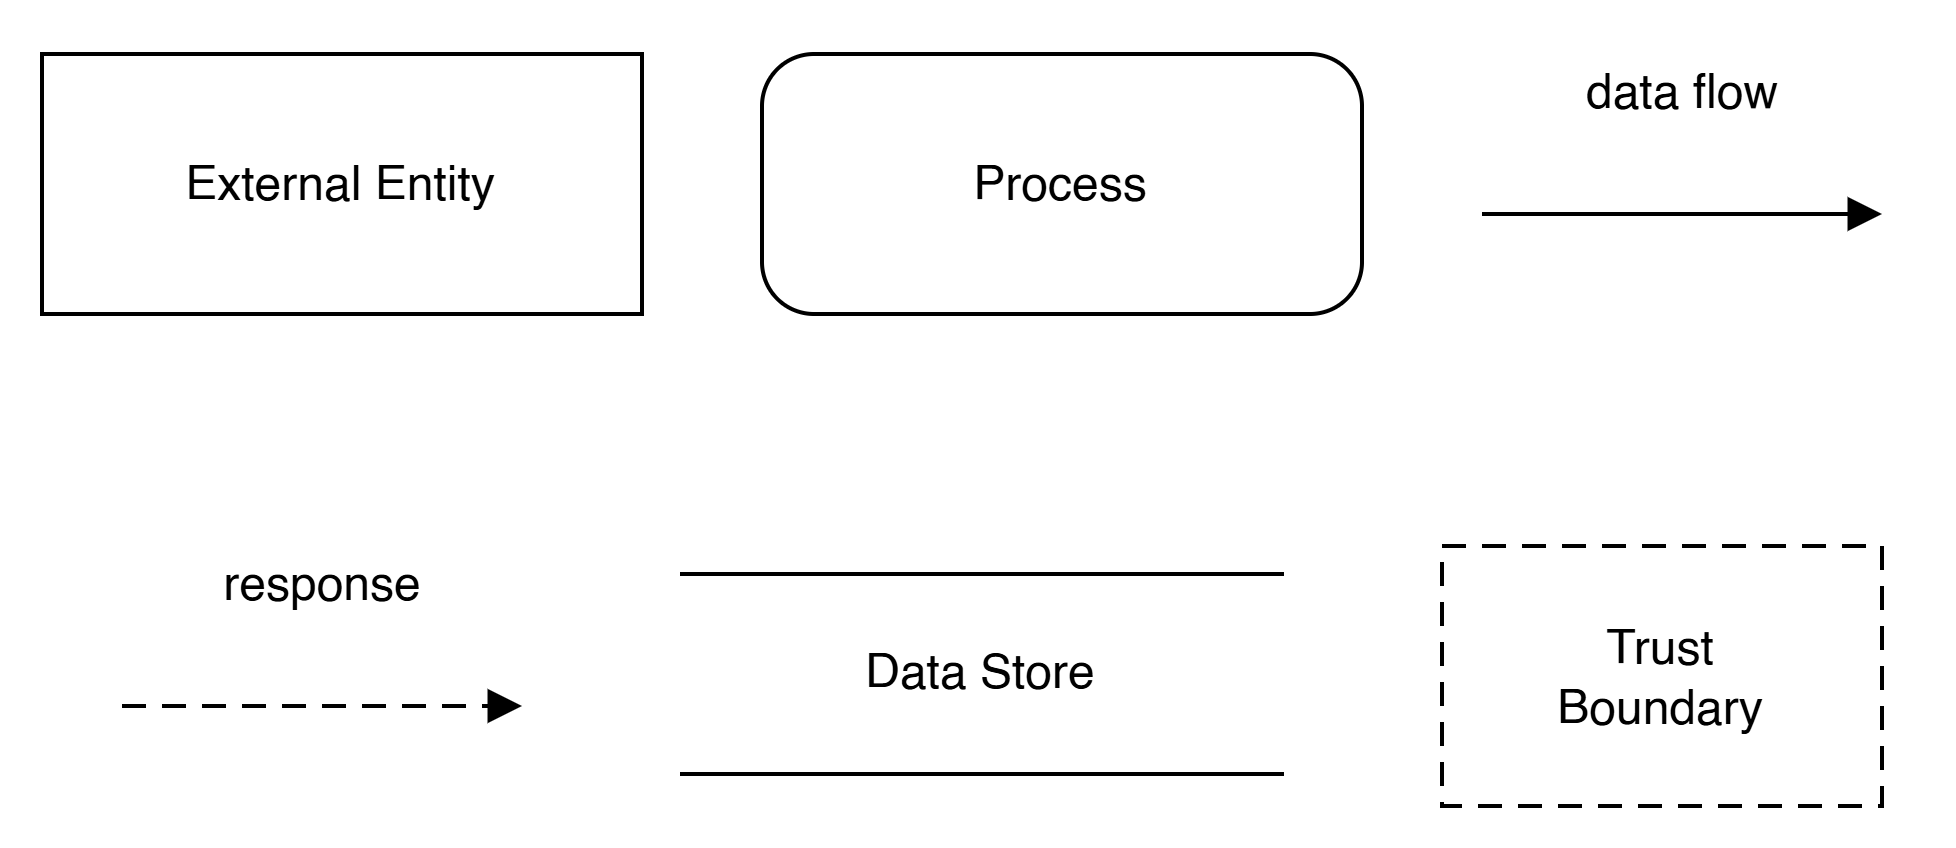
\includegraphics[width=1\textwidth]{resources/appendix/legenda-dfd.png}
	\caption{Legenda \textit{Data Flow Diagram} (Dokumentasi Penulis)}
	\label{fig:legenda-dfd}
\end{figure}

\begin{figure}[ht]
	\centering
	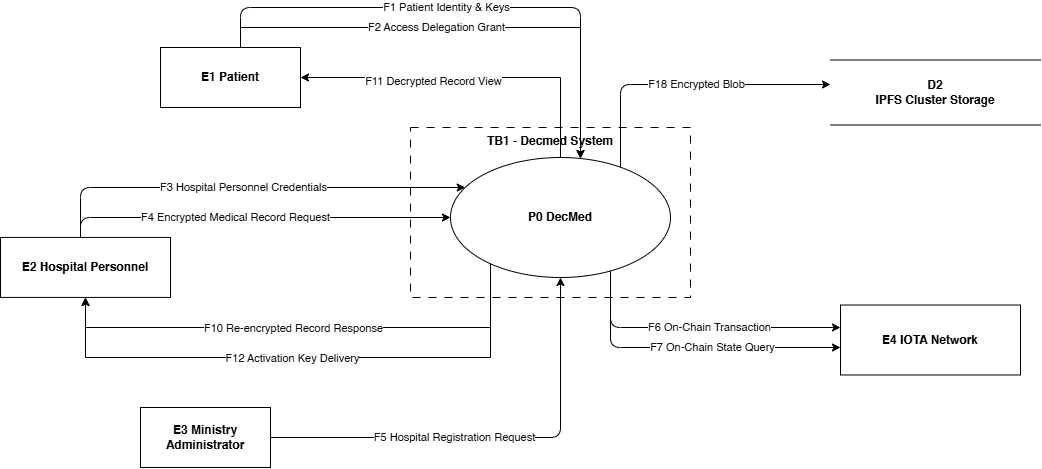
\includegraphics[width=1\textwidth]{resources/chapter-3/analisis/DFD-DecMed-Level-0.png}
	\caption{DFD DecMed Level 0 (Dokumentasi Penulis)}
	\label{fig:dfd-decmed-level-0}
\end{figure}

\begin{landscape}
	\begin{figure}[ht]
		\centering
		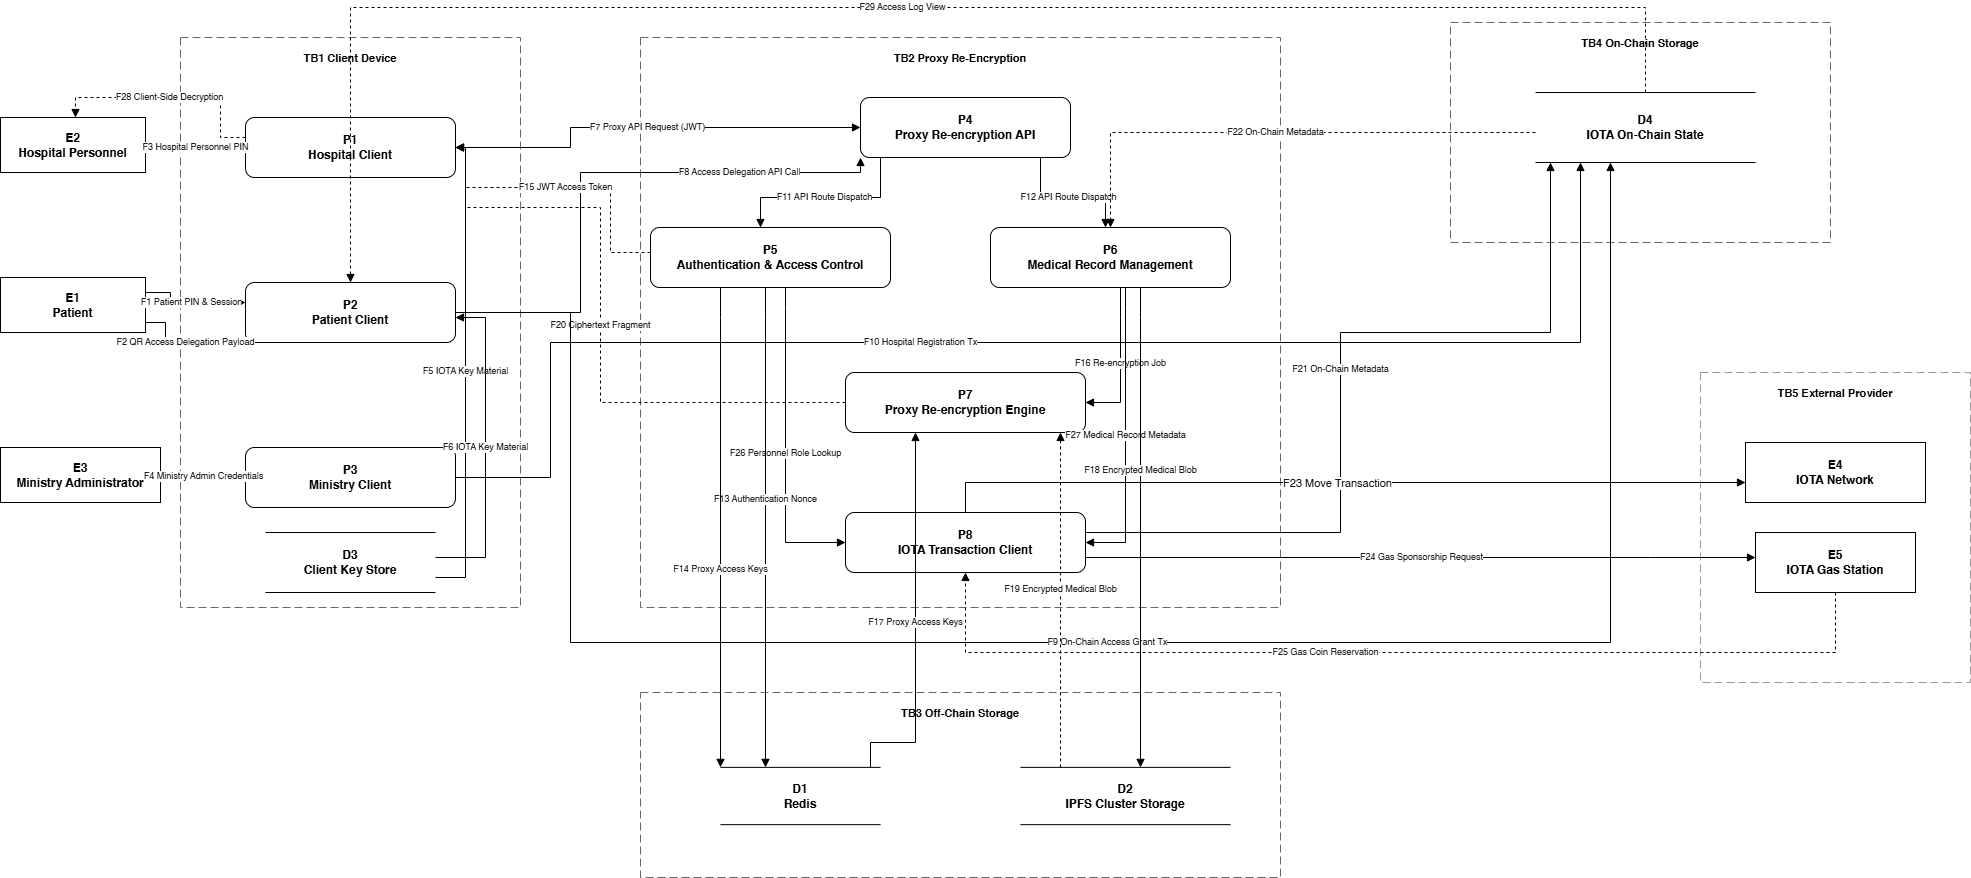
\includegraphics[height=0.80\textheight]{resources/chapter-3/analisis/DFD-DecMed-Level-1.png}
		\caption{DFD DecMed Level 1 (Dokumentasi Penulis)}
		\label{fig:dfd-decmed-level-1}
	\end{figure}
\end{landscape}

\begin{table}[!ht]
	\centering
	\caption{Daftar \textit{External Entities} pada DFD DecMed}
	\label{tab:dfd-external-entities}
	\small
	\begin{tabular}{|p{0.10\textwidth}|p{0.22\textwidth}|p{0.58\textwidth}|}
		\hline
		\textbf{ID} & \textbf{Nama}          & \textbf{Interaksi utama}                                                  \\ \hline
		E1          & Patient                & PIN, QR delegasi akses, \textit{revoke access}, lihat \textit{access log} \\ \hline
		E2          & Hospital Personnel     & PIN, baca/\textit{update} rekam medis, data administratif                 \\ \hline
		E3          & Ministry Administrator & Registrasi rumah sakit, \textit{activation key}                           \\ \hline
		E4          & IOTA Network           & RPC, \textit{publish/execute transaction}, \textit{read state}            \\ \hline
		E5          & IOTA Gas Station       & \texttt{reserve\_gas}, \texttt{execute\_tx}                               \\ \hline
	\end{tabular}
\end{table}

\begin{table}[!ht]
	\centering
	\caption{Daftar \textit{Process} DFD DecMed}
	\label{tab:dfd-process}
	\small
	\begin{tabular}{|p{0.06\textwidth}|p{0.5\textwidth}|}
		\hline
		\textbf{ID} & \textbf{Nama}                    \\ \hline
		P0          & Decmed (seluruh sistem)          \\ \hline
		P1          & Hospital Client                  \\ \hline
		P2          & Patient Client                   \\ \hline
		P3          & Ministry Client                  \\ \hline
		P4          & Proxy Re-encryption API          \\ \hline
		P5          & Authentication \& Access Control \\ \hline
		P6          & Medical Record Management        \\ \hline
		P7          & Proxy Re-encryption Engine       \\ \hline
		P8          & IOTA Transaction Client          \\ \hline
	\end{tabular}
\end{table}

\begin{table}[!ht]
	\centering
	\caption{Daftar \textit{Data Store} pada DFD DecMed}
	\label{tab:dfd-data-store}
	\small
	\begin{tabular}{|p{0.08\textwidth}|p{0.28\textwidth}|p{0.52\textwidth}|}
		\hline
		\textbf{ID} & \textbf{Nama}        & \textbf{Data sensitif}                                                                    \\ \hline
		D1          & Redis Cache          & \textit{Nonce challenge}, \texttt{AccessKeys} (k-frag, PRE public keys, seed terenkripsi) \\ \hline
		D2          & IPFS Cluster Storage & Blob rekam medis terenkripsi (CID direferensikan \textit{on-chain})                       \\ \hline
		D3          & Client OS Keyring    & IOTA keypair, PRE keys, PIN-derived secrets, \textit{activation key}                      \\ \hline
		D4          & IOTA On-Chain State  & Metadata, \textit{access grants}, \textit{access log}, \textit{hospital registry}         \\ \hline
	\end{tabular}
\end{table}

\begin{table}[!ht]
	\centering
	\caption{Daftar Data Flow pada DFD DecMed (Level 0)}
	\label{tab:dfd-dataflow-level-0}
	\small
	\begin{tabular}{|p{0.06\textwidth}|p{0.39\textwidth}|p{0.24\textwidth}|}
		\hline
		\textbf{ID} & \textbf{Label}                   & \textbf{Arah}       \\ \hline
		F1          & Patient Identity \& Keys         & E1~$\rightarrow$~P0 \\ \hline
		F2          & Access Delegation Grant          & E1~$\rightarrow$~P0 \\ \hline
		F3          & Hospital Personnel Credentials   & E2~$\rightarrow$~P0 \\ \hline
		F4          & Encrypted Medical Record Request & E2~$\rightarrow$~P0 \\ \hline
		F5          & Hospital Registration Request    & E3~$\rightarrow$~P0 \\ \hline
		F6          & On-Chain Transaction             & P0~$\rightarrow$~E4 \\ \hline
		F7          & On-Chain State Query             & P0~$\rightarrow$~E4 \\ \hline
		F10         & Re-encrypted Record Response     & P0~$\rightarrow$~E2 \\ \hline
		F11         & Decrypted Record View            & P0~$\rightarrow$~E1 \\ \hline
		F12         & Activation Key Delivery          & P0~$\rightarrow$~E2 \\ \hline
		F18         & Encrypted Blob                   & P0~$\rightarrow$~D2 \\ \hline
	\end{tabular}
\end{table}

\begin{table}[!ht]
	\centering
	\caption{Daftar Data Flow pada DFD DecMed (Level 1)}
	\label{tab:dfd-dataflow-level-1}
	\small
	\begin{tabular}{|p{0.08\textwidth}|p{0.43\textwidth}|p{0.31\textwidth}|}
		\hline
		\textbf{ID} & \textbf{Label}               & \textbf{Arah Ringkas} \\ \hline
		F1          & Patient PIN \& Session       & E1~$\rightarrow$~P2   \\ \hline
		F2          & QR Access Delegation Payload & E1~$\rightarrow$~P2   \\ \hline
		F3          & Hospital Personnel PIN       & E2~$\rightarrow$~P1   \\ \hline
		F4          & Ministry Admin Credentials   & E3~$\rightarrow$~P3   \\ \hline
		F5          & IOTA Key Material            & D3~$\rightarrow$~P1   \\ \hline
		F6          & IOTA Key Material            & D3~$\rightarrow$~P2   \\ \hline
		F7          & Proxy API Request (JWT)      & P1~$\rightarrow$~P4   \\ \hline
		F8          & Access Delegation API Call   & P2~$\rightarrow$~P4   \\ \hline
		F9          & On-Chain Access Grant Tx     & P2~$\rightarrow$~D4   \\ \hline
		F10         & Hospital Registration Tx     & P3~$\rightarrow$~D4   \\ \hline
		F11         & API Route Dispatch           & P4~$\rightarrow$~P5   \\ \hline
		F12         & API Route Dispatch           & P4~$\rightarrow$~P6   \\ \hline
		F13         & Authentication Nonce         & P5~$\rightarrow$~D1   \\ \hline
		F14         & Proxy Access Keys            & P5~$\rightarrow$~D1   \\ \hline
		F15         & JWT Access Token             & P5~$\rightarrow$~P1   \\ \hline
		F16         & Re-encryption Job            & P6~$\rightarrow$~P7   \\ \hline
		F17         & Proxy Access Keys            & D1~$\rightarrow$~P7   \\ \hline
		F18         & Encrypted Medical Blob       & P6~$\rightarrow$~D2   \\ \hline
		F19         & Encrypted Medical Blob       & D2~$\rightarrow$~P7   \\ \hline
		F20         & Ciphertext Fragment          & P7~$\rightarrow$~P1   \\ \hline
		F21         & On-Chain Metadata            & P8~$\rightarrow$~D4   \\ \hline
		F22         & On-Chain Metadata            & D4~$\rightarrow$~P6   \\ \hline
		F23         & Move Transaction             & P8~$\rightarrow$~E4   \\ \hline
		F24         & Gas Sponsorship Request      & P8~$\rightarrow$~E5   \\ \hline
		F25         & Gas Coin Reservation         & E5~$\rightarrow$~P8   \\ \hline
		F26         & Personnel Role Lookup        & P5~$\rightarrow$~P8   \\ \hline
		F27         & Medical Record Metadata      & P6~$\rightarrow$~P8   \\ \hline
		F28         & Client-Side Decryption       & P1~$\rightarrow$~E2   \\ \hline
		F29         & Access Log View              & D4~$\rightarrow$~P2   \\ \hline
	\end{tabular}
\end{table}
